\chapter{Wat is bitcoin?}

Bitcoin is een vorm van \textit{peer-to-peer elektronisch geld}, een vernieuwend soort digitaal geld dat kan worden overgemaakt tussen personen of computers zonder enige vertrouwde tussenpersoon (zoals een bank), en waarvan de uitgifte niet onder controle staat van één enkele partij. 

Denk maar eens aan een papieren dollarbiljet of een fysieke metalen munt. Als je deze aan iemand geeft, is het niet nodig dat die persoon weet wie je bent. Ze hoeven alleen maar te vertrouwen dat het geld dat ze ontvangen geen vervalsing is. Bij fysiek geld vertrouwen mensen over het algemeen op hun ogen en tastzin, of bij grotere hoeveelheden op speciale apparatuur om echt geld van vervalsingen te onderscheiden.

Maar in onze digitale samenleving verlopen de meeste van onze betalingen via een tussenpersoon: of het nu via een bank is met behulp van \textit{iDeal}, een creditcardmaatschappij zoals \textit{Visa}, een digitale betalingsdienst zoals \textit{PayPal}, of \textit{WeChat} in China.

Met de overgang naar de digitale wereld is geld veranderd van een fysiek iets dat je zelf kunt bijhouden, overdragen en verifiëren, naar digitale bits die door een derde partij worden opgeslagen, geverifieerd en verstuurd. Daardoor ben je voor elke digitale financiële handeling nu afhankelijk van een derde partij. 

Doordat we contant geld opgeven voor het gemak van digitale betalingen, geven we tegelijkertijd anderen buitengewone macht om ons te onderdrukken. Digitale betaalplatformen zijn verworden tot de basis van dystopische, autoritaire controlesystemen. Een voorbeeld hiervan is de Chinese overheid, die deze systemen inzet om dissidenten te controleren en bepaalde burgers te belemmeren in het gebruik van goederen of diensten.

Bitcoin biedt een alternatief voor centraal gestuurd, digitaal geld. Het geeft ons een systeem dat de vrijheid van fysiek geld terugbrengt, maar dan in digitale vorm:

\begin{enumerate}
    \item Een digitaal bezit met een beperkt, vooraf bepaald en onveranderlijk aanbod. Dit staat in schril contrast met bankbiljetten en hun digitale varianten uitgegeven door overheden en centrale banken, waarvan de hoeveelheid zich onvoorspelbaar blijft vermeerderen.
    \item  	Een netwerk van met elkaar verbonden computers, het zogenaamde bitcoinnetwerk, waar iedereen aan kan deelnemen door een bepaalde software op hun computer te installeren. Dit netwerk maakt het mogelijk om bitcoins uit te geven, de eigendomsrechten ervan te traceren en transacties tussen deelnemers uit te voeren. Dit alles zonder de tussenkomst of het vertrouwen in bemiddelaars zoals banken, betalingsdiensten of overheidsinstellingen.
    \item  	De bitcoincliëntsoftware, een stukje computercode die iedereen kan gebruiken om deel uit te maken van het netwerk. Deze software is \textit{open-source}, hetgeen betekent dat iedereen de werking ervan kan inzien en kan bijdragen aan nieuwe functies en verbeteringen.

\end{enumerate}
\begin{figure}[h]
    \centering
    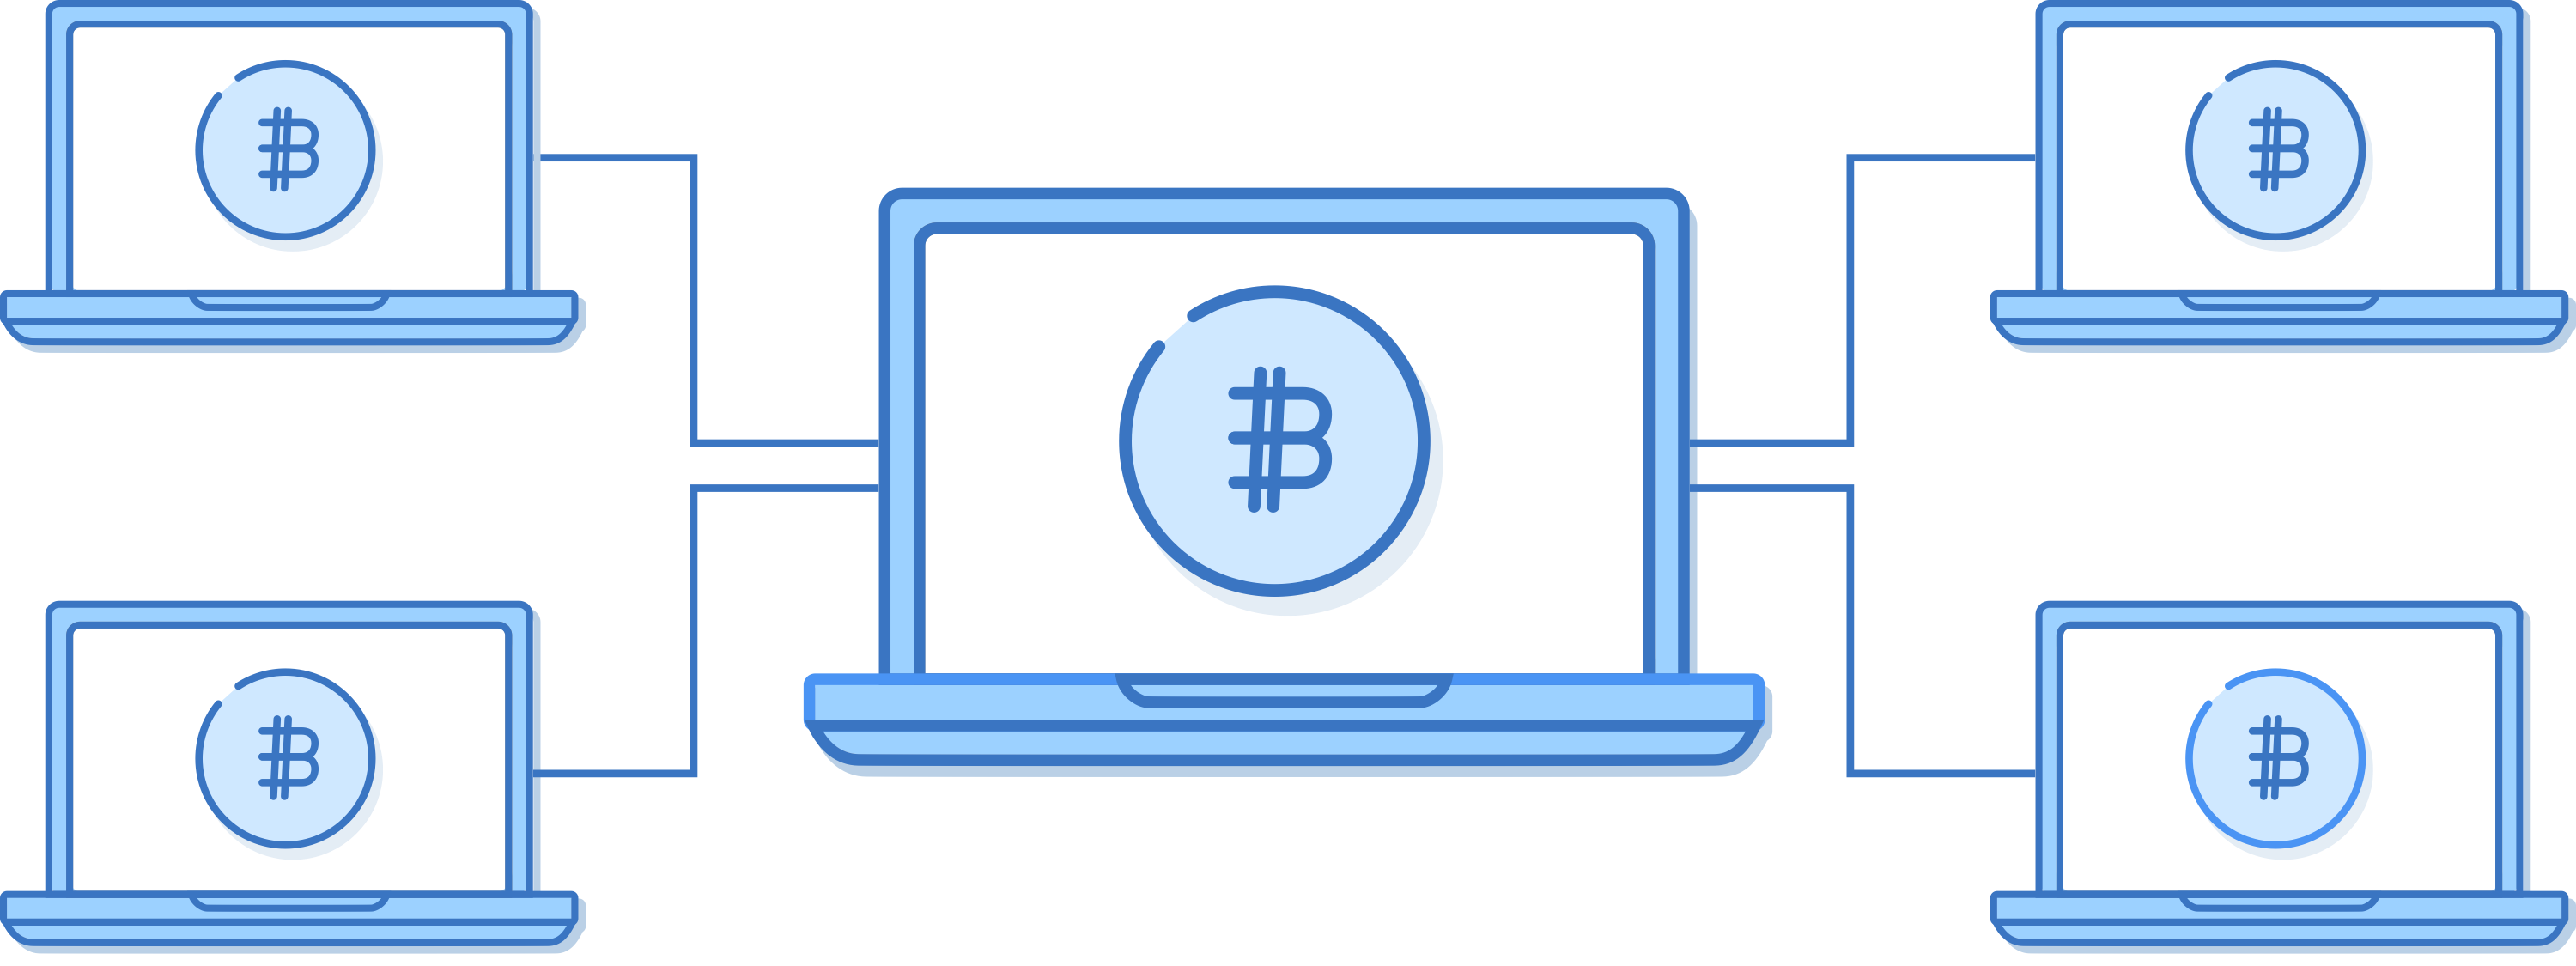
\includegraphics[width=\textwidth]{images/fig1.png}
    \caption{\footnotesize{\textit{Bitcoin is een netwerk van computers die de bitcoincliëntsoftware draaien}.}}
    \label{fig1}
\end{figure}

\noindent Later in het boek zullen we dieper ingaan op wat de drijfveren achter bitcoin zijn.

\clearpage
\section{Waar komt bitcoin vandaan?}

Bitcoin is rond 2008 uitgevonden door een of meer personen die bekend staan onder het pseudoniem  \href{https://nl.wikipedia.org/wiki/Satoshi_Nakamoto}{\textbf{Satoshi Nakamoto}}\footnote{Binnen de gemeenschap wordt naar Satoshi vaak verwezen als een man. In dit boek zullen we ook op deze manier naar hem verwijzen, ondanks dat we niet weten of het in werkelijkheid om een man, vrouw of een groep mensen gaat.}. Niemand kent de identiteit van Satoshi, en voor zover we weten is hij verdwenen en heeft hij al jaren niets meer van zich laten horen.

Op 11 februari 2009 vertelde Satoshi op een online forum, bestemd voor mensen die zich bezighouden met cryptografie en die grote waarde toekennen aan individuele privacy en vrijheid – de zogenaamde \textit{cypherpunks} – over een vroege versie van bitcoin. Hoewel dit niet de eerste officiële aankondiging van bitcoin was, verschaft het wel een uitstekende samenvatting van Satoshi's drijfveren. Daarom wil ik dit gebruiken als basis voor onze discussie.

Ik zal een aantal citaten aanhalen die duidelijk maken welke problemen Satoshi probeerde op te lossen in het huidige financiële systeem:

\begin{quote}
\textit{Ik heb een nieuw open-source P2P e-cash systeem ontwikkeld genaamd bitcoin. Het is volledig gedecentraliseerd, zonder centrale server of vertrouwde partijen. alles berust op cryptografisch bewijs in plaats van op vertrouwen. [...]}

\textit{Het kernprobleem met conventionele valuta is het vertrouwen dat nodig is om het te laten werken. We moeten de centrale bank vertrouwen [om de valuta niet te devalueren], maar de geschiedenis van fiatvaluta is doordrenkt met schendingen van dit vertrouwen. We moeten banken vertrouwen om ons geld veilig te bewaren en elektronisch over te boeken, maar zij lenen het uit in golven van kredietbubbels met slechts een fractie van die waarde als reserve. We moeten ze onze privacy toevertrouwen en we moeten erop vertrouwen dat ze identiteitsdieven kunnen stoppen die onze rekeningen willen plunderen. Hun hoge overheadkosten maken microbetalingen onmogelijk.}

\textit{Eerder kampten \textit{multi-user time-sharing} computersystemen met een soortgelijk probleem. Voor robuuste encryptie moesten gebruikers nog steeds terugvallen op wachtwoorden om hun bestanden te beschermen [...]}

\textit{Toen sterke encryptie voor iedereen beschikbaar werd, werd vertrouwen overbodig. Gegevens konden beveiligd worden zodat niemand er toegang toe kon krijgen, ongeacht de reden, hoe goed het excuus ook was, wat er ook gebeurde.}

\textit{Het is hoog tijd dat we dit ook kunnen realiseren voor geld. Doormiddel van een e-valuta die gebaseerd is op cryptografisch bewijs, zonder dat we afhankelijk zijn van een tussenpersoon. Geld kan veilig zijn en transacties kunnen zonder enige moeite worden uitgevoerd. [...]}

\textit{De oplossing van bitcoin is om een peer-to-peer-netwerk te gebruiken om te controleren op dubbele uitgaven. In een notendop werkt het netwerk als een gedistribueerde tijdstempel, die de eerste uitgave van een munt markeert met een tijdsaanduiding. Hierbij wordt er gebruik gemaakt van het feit dat informatie eenvoudig te verspreiden is, maar lastig te stoppen.}

\textit{Voor meer informatie over hoe het werkt, zie het ontwerpdocument op \href{http://www.bitcoin.org/bitcoin.pdf}{http://www.bitcoin.org/bitcoin.pdf}.}
\par\raggedleft--- \textup{SATOSHI NAKAMOTO}
\end{quote}

\section{Welke problemen lost het op?}

Laten we eens wat dieper ingaan op een aantal beweringen van Satoshi. In de loop van dit boek zullen we uitgebreid bespreken hoe deze concepten in de praktijk worden gebracht. Maak je geen zorgen als je iets in dit hoofdstuk nog niet helemaal begrijpt; we zullen er later op terugkomen. Het idee is om de beweegredenen van Satoshi te begrijpen, zodat we deze later in het boek verder kunnen onderzoeken.

\begin{quote}
\textit{Ik heb een nieuw open source P2P e-cash systeem ontwikkeld}
\end{quote}

P2P is de afkorting van \textit{peer-to-peer}, wat verwijst naar een systeem waarbij de ene persoon rechtstreeks interactie heeft met de ander, zonder tussenkomst van een derde partij. Beide partijen (de ontvanger en de verzender) zijn gelijkwaardig aan elkaar. Misschien herinner je je nog P2P-technologieën zoals \textit{Napster}, \textit{Kazaa} en \textit{BitTorrent}, waarmee mensen voor het eerst direct bestanden, muziek en films met elkaar konden delen zonder een tussenpersoon. Satoshi ontwierp bitcoin met het idee om mensen op nagenoeg dezelfde manier elektronisch geld (e-cash) te laten uitwisselen, wederom zonder bemiddeling van een derde partij.

De software is \textit{open source}, wat inhoudt dat iedereen de werking ervan kan zien en bijdragen kan leveren. Dit is van groot belang aangezien het voor transparantie zorgt. Er is geen vertrouwen voor nodig. We hoeven niet klakkeloos aan te nemen wat Satoshi in zijn berichten over de werking van de software heeft geschreven. We hebben de mogelijkheid om de code zelf te bestuderen en te controleren hoe het allemaal in elkaar zit. Daarnaast bestaat er de mogelijkheid om de functionaliteit van het systeem te verbeteren door eigen aanpassingen in de code door te voeren.

\begin{quote}
\textit{Het is volledig gedecentraliseerd, zonder centrale server of vertrouwde partijen...}
\end{quote}

Satoshi benadrukt dat het systeem \textit{gedecentraliseerd} is om zich te onderscheiden van systemen die wel een centrale sturing hebben. Eerdere pogingen om digitaal contant geld te creëren, zoals \textit{DigiCash} van David Chaum, werden gefaciliteerd door een centrale server; een computer of reeks computers die verantwoordelijk waren voor de uitgifte en verificatie van betalingen, \textit{onder het beheer van één enkel bedrijf}.

Dit soort particuliere, centraal gestuurde digitale valuta zijn gedoemd te falen. We kunnen ons geld niet toevertrouwen aan een systeem dat kan instorten als een bedrijf failliet gaat, gehackt wordt, IT-problemen ondervindt of door de overheid wordt stilgelegd.

Bitcoin, aan de andere kant, wordt niet beheerd en gecontroleerd door slechts één bedrijf, maar door een netwerk van individuen en bedrijven over de hele wereld. Het zou een onmogelijke opgave zijn om bitcoin stop te zetten, want dat zou inhouden dat je tienduizenden tot honderdduizenden computers wereldwijd zou moeten stilleggen, waarvan vele moeilijk op te sporen zijn Het is een hopeloos kat-en-muisspel aangezien elke aanval van deze aard eenvoudigweg de creatie van nieuwe \textit{bitcoin-nodes} of computers op het netwerk aanmoedigt.

\begin{quote}
\textit{ ... alles berust op cryptografisch bewijs in plaats van op vertrouwen.}
\end{quote}

Het internet en de meeste hedendaagse computersystemen zijn gebaseerd op cryptografie; een techniek waarbij informatie wordt versleuteld zodat alleen de bedoelde ontvanger deze kan ontcijferen. Hoe ontsnapt bitcoin aan de noodzaak van \textit{vertrouwen}? We zullen dit later in het boek uitvoerig behandelen, maar de kern van het idee is dat we in plaats van iemand te geloven die beweert ``Ik ben Alice'' of ``Ik heb €10 op mijn rekening'', cryptografie kunnen aanwenden om dergelijke feiten te presenteren op een manier waarbij de ontvanger het bericht zelf eenvoudig kan verifiëren en het onmogelijk is om te vervalsen. Bitcoin gebruikt cryptografie om deelnemers in staat te stellen het gedrag van alle anderen te controleren, zonder dat hierbij een centrale partij vertrouwt hoeft te worden.

\begin{quote}
\textit{We moeten ze [de banken] onze privacy toevertrouwen, en erop vertrouwen dat zij identiteitsdieven kunnen beletten om onze rekeningen leeg te halen}
\end{quote}

In tegenstelling tot het gebruik van een bankrekening, het digitale betalingssysteem of kredietkaarten, stelt bitcoin twee partijen in staat om transacties uit te voeren zonder persoonlijke identificatie op te geven. Banken, kredietkaartmaatschappijen, betalingsverwerkers en overheden beschikken over gecentraliseerde databanken van consumentengegevens. Deze informatie is een potentiële goudmijn voor hackers. Neem bijvoorbeeld de hack van \textit{Equifax} in 2017, waarbij de identiteits- en financiële gegevens van meer dan 140 miljoen mensen gestolen werden. Dit soort databases en de daarmee verbonden hacks kunnen leiden tot grootschalige identiteitsfraude.

Bitcoin maakt financiële transacties los van onze werkelijke identiteit. Immers, wanneer we iemand contant geld geven, heeft de ontvanger niet noodzakelijk onze identiteit nodig, en hoeft degene die betaalt niet bang te zijn dat zijn gegevens later worden gebruikt om hem te beroven. Waarom zouden we niet hetzelfde, of zelfs meer, mogen verwachten van digitaal geld?

\begin{quote}
\textit{We moeten de centrale bank vertrouwen [om de valuta niet te devalueren], maar de geschiedenis van fiatvaluta is doordrenkt met schendingen van dit vertrouwen.}
\end{quote}

\textit{Fiat}, wat ``laat het gebeuren'' betekent in het Latijn, verwijst naar de door de overheid en de centrale bank uitgegeven valuta, die door de overheid als wettig betaalmiddel wordt erkend. In de geschiedenis werd geld vaak gemaakt uit materialen die moeilijk te produceren, eenvoudig te verifiëren en gemakkelijk te vervoeren waren, zoals schelpen, glaskralen, zilver en goud. Telkens als iets als geld werd ingezet, ontstond de verleiding om er meer van te produceren. Als iemand aan kwam zetten met geavanceerde technologie om snel veel van iets te maken, verloor het voorwerp zijn waarde. Op deze manier konden Europese kolonisten Afrika beroven van haar rijkdommen door te handelen met glaskralen, die gemakkelijk waren voor de Europeanen maar moeilijk voor de Afrikanen om te vervaardigen. Dit is waarom goud al lange tijd wordt gezien als een betrouwbare vorm van geld -- het is immers moeilijk om snel goud te produceren.\footnote{Voor een goed overzicht van de monetaire geschiedenis raad ik het essay \textit{Shelling Out} van Nick Szabo aan: \href{https://nakamotoinstitute.org/shelling-out}{https://nakamotoinstitute.org/shelling-out}}

We zijn geleidelijk overgestapt van een wereldwijde economie waarin goud als geld diende, naar een systeem waar papieren certificaten uitgegeven werden als recht, of vordering, op datzelfde goud. Uiteindelijk koppelde president Nixon deze papieren claims volledig los van het goud. In 1971 maakte hij een einde aan de internationale mogelijkheid om de Amerikaanse dollar in te wisselen voor goud.

Het einde van de goudstandaard stelde overheden en centrale banken in staat om de geldhoeveelheid naar believen te vergroten, waardoor ieder biljet in omloop minder waard werd. Dit fenomeen staat bekend als \textit{geldontwaarding}. Hoewel een fiatvaluta wordt uitgegeven door een overheid, het tegen niets inwisselbaar is, en we het dagelijks gebruiken, is het eigenlijk een relatief recent experiment in de geschiedenis van de wereld.

We moeten erop vertrouwen dat onze overheden de macht over de geldvoorziening niet misbruiken. Maar we hoeven niet ver te zoeken om voorbeelden te vinden waarbij dat vertrouwen ernstig is geschonden. Dit komt voornamelijk voor in autocratische regimes, waar de regering directe controle heeft over de geldpers. Een sprekend voorbeeld is Venezuela, waar de munteenheid praktisch waardeloos is geworden. De Venezolaanse bolivar is gestegen van 2 bolivar per Amerikaanse dollar in 2009, naar maar liefst 250.000 bolivar per Amerikaanse dollar in 2019. Terwijl ik dit boek schrijf, is de ineenstorting van Venezuela volop aan de gang als gevolg van het vreselijke economische wanbeleid van de regering.

Satoshi wilde een alternatief creëren voor fiatgeld, waarvan de hoeveelheid te allen tijde onvoorspelbaar kan worden verhoogd. Om devaluatie te voorkomen, bedacht hij een geldsysteem waarin de totale voorraad op voorhand is vastgelegd en de uitgifte van nieuwe munten een voorspelbaar en onwrikbaar patroon volgt. Er zullen slechts 21 miljoen bitcoins bestaan en elke bitcoin kan worden opgesplitst in 100 miljoen eenheden, nu bekend als satoshis. In de code is vastgelegd dat rond het jaar 2140 het eindtotaal bereikt wordt van 2,1 biljard satoshis.

Tot bitcoin was het onmogelijk om te verkomen dat een digitaal product oneindig werd gekopieerd. Het is goedkoop en eenvoudig om een digitaal boek, audiobestand of videobestand te kopiëren en door te sturen. De enige uitzonderingen hierop waren digitale producten die beheerd werden door tussenpersonen. Neem bijvoorbeeld Netflix: als je een film via dit platform bekijkt, kun je deze alleen op je eigen apparaat bekijken omdat Netflix de film levert. Je kunt deze film niet zelf verspreiden of kopiëren. Op dezelfde wijze beheert de bank je digitale geld. De bank is verantwoordelijk om bij te houden hoeveel geld je hebt, en als je geld aan iemand anders overmaakt, regelt de bank die\footnote{Ze zijn dus ook in staat deze te weigeren}

Bitcoin vormt het eerste digitale systeem dat schaarste kan creëren zonder de noodzaak van tussenpersonen. Daarnaast is het ook het eerste goed waarvan het totale aanbod en het emissieschema bij voorbaat bekend is. Zelfs edelmetalen zoals goud kennen deze eigenschap niet omdat we simpelweg meer goud kunnen delven als het winstgevend is dit te doen. Stel je eens voor dat je een asteroïde ontdekt met tien keer zoveel goud als er op aarde is. Wat zou er dan gebeuren met de goudprijs? Geen zorgen, bitcoin is resistent tegen dergelijke ontdekkingen. Het is onmogelijk om er meer van te produceren, en we leggen in latere hoofdstukken uit waarom.
 
De aard van geld en de werking van het bestaande monetaire systeem zijn ingewikkeld. Dit boek gaat hier niet dieper op in. Als je hier meer over wilt weten in de context van bitcoin, dan raad ik \textit{De Bitcoin Standaard} van Saifedean Ammous aan.
\clearpage
\begin{quote}
\textit{Gegevens konden beveiligd worden zodat niemand er toegang toe kon krijgen, ongeacht de reden, hoe goed het excuus ook was, wat er ook gebeurde. [...]
Het is hoog tijd dat we dit ook kunnen realiseren voor geld.} 
\end{quote}

Onze huidige methoden om geld veilig te bewaren, zoals het storten op een bankrekening, zijn afhankelijk van het feit dat derden hun werk correct uitvoeren. Vertrouwen op een derde partij betekent niet alleen dat we moeten geloven dat zij geen kwaad of stommiteiten begaan, maar ook dat de overheid hen niet onder druk zet om dergelijke handelingen te verrichten. Het gaat hierbij bijvoorbeeld om situaties waarin iemand de toegang tot zijn geld wordt ontnomen of het geld wordt geconfisqueerd. Helaas is uit ervaring gebleken dat overheden, wanneer ze zich bedreigd voelen of een bedreiging waarnemen, in staat zijn en bereid kunnen zijn om dergelijke acties te ondernemen en door te voeren.

Het kan misschien vreemd klinken voor iemand die in de Verenigde Staten (of in een andere sterk gereguleerde economie) woont, maar stel je voor dat je wakker wordt en ineens al je geld kwijt bent. Deze situaties komen vaker voor dan je zou denken. Ik heb dit zelf meegemaakt toen mijn PayPal-rekening bevroren werd omdat ik deze al maandenlang niet had gebruikt. Het kostte me ruim een week om weer toegang tot ``mijn'' geld te krijgen. Gelukkig woon ik in de Verenigde Staten, waar ik tenminste juridische bijstand kan inschakelen als \textit{PayPal} mijn saldo bevriest, en waar ik er over het algemeen vanuit kan gaan dat mijn overheid en de bank mijn geld niet zullen inpikken.

Er zijn in het verleden, en vandaag nog steeds, veel ergere dingen gebeurd in landen met minder vrijheid, zoals banken die sluiten tijdens de crisis in Griekenland (2015)\footnote{\href{https://www.nbcnews.com/business/business-news/greece-crisis-banks-shut-week-restrictions-imposed-atms-n383606}{https://nbcnews.com/business/business-news/greece-crisis-banks-shut-week-restrictions-imposed-atms-n383606}}, banken in Cyprus die via bail-ins het geld van hun klanten in beslag nemen (2013), of de overheid die bepaalde bankbiljetten waardeloos verklaart in India (2016)\footnote{\href{https://www.washingtonpost.com/world/asia\_pacific/india-invalidates-large-bank-notes-in-crackdown-on-crime/2016/11/08/cc705ee2-a5c6-11e6-ba46-53db57f0e351\_story.html}{https://www.washingtonpost.com/world/asia\_pacific/india-invalidates-large-bank-notes-in-crackdown-on-crime/2016/11/08/cc705ee2-a5c6-11e6-ba46-53db57f0e351\_story.html}}.

Ik ben opgegroeid in wat vroeger de Sovjet-Unie was. Daar had de overheid de controle over de economie, wat resulteerde in ernstige tekorten aan goederen. Het bezit van buitenlandse valuta's zoals de Amerikaanse dollar was illegaal. Toen mijn ouders besloten te vertrekken, konden we per persoon slechts een beperkt bedrag omzetten naar dollars. De door de overheid vastgestelde wisselkoers lag ver van de marktwisselkoers. In feite heeft de regering ons beroofd van het beetje vermogen dat we hadden, door een strakke greep op de economie en het betalingsverkeer te houden.

Autocratische landen hebben de neiging om strenge economische controles in te voeren om te voorkomen dat mensen hun geld uit banken opnemen, het land uitvoeren of inruilen voor nog-niet-waardeloze valuta zoals de Amerikaanse dollar. Hierdoor heeft de regering vrij spel om krankzinnige economische experimenten, zoals het socialistische systeem van de Sovjet-Unie, uit te voeren.

Bitcoin werkt niet op basis van vertrouwen in een derde partij voor het veilig stellen van je geld. In plaats daarvan maakt bitcoin het \textit{onmogelijk} voor anderen om toegang te krijgen zonder een speciale sleutel die alleen de eigenaar bezit, \textit{ongeacht om welke reden, ongeacht hoe goed het excuus, wat er ook gebeurt}. Door bitcoin te bezitten, bezit je de sleutels van je eigen financiële vrijheid. Bitcoin scheidt geld en staat.

\begin{quote}
\textit{De oplossing die bitcoin aandraagt is het gebruik van een peer-to-peer-netwerk om dubbele uitgaven te controleren [...] als een gedistribueerde tijdstempel, waarbij de eerste uitgave van een munt van een tijdstempel wordt voorzien.}
\end{quote}

Een \textit{netwerk} verwijst naar het idee dat een stel computers zijn verbonden en informatie naar elkaar kunnen sturen. Het woord \textit{gedistribueerd} betekent dat er geen centrale partij aan de macht is, maar dat alle deelnemers samenwerken om het netwerk succesvol te maken.

Binnen een systeem zonder gecentraliseerde controle, is het cruciaal dat niemand vals kan spelen. Het concept van ``double spending'' -- oftewel \textit{dubbele uitgaven} -- verwijst naar de mogelijkheid om tweemaal hetzelfde geld uit te geven. Dit is geen probleem met fysiek geld, aangezien dit van eigenaar wisselt zodra je het uitgeeft. Digitale transacties, daarentegen, kunnen gekopieerd worden, net zoals muziek of films. Wanneer je geld overmaakt via een bank, zorgt de bank ervoor dat je niet tweemaal hetzelfde geld kunt verplaatsen. In een systeem zonder gecentraliseerde controle, hebben we een oplossing nodig om dit soort dubbele uitgaven te vermijden (dubbele uitgaven komen overeen met valsemunterij).

Satoshi beschrijft dat de deelnemers van het bitcoinnetwerk samenwerken om transacties van \textit{tijdstempels} te voorzien. Door deze tijdstempel weten we welke transactie eerst kwam zodat we toekomstige pogingen om datzelfde geld uit te geven afwijzen. In de volgende hoofdstukken zullen we dit systeem vanaf de basis bespreken. Het zal ons in staat stellen om vals spel te detecteren zonder te vertrouwen op een centrale uitgever of validator.

Bitcoin was geen uitvinding die op zichzelf stond. In de paper noemde Satoshi verschillende belangrijke pogingen om soortgelijke systemen te implementeren, waaronder Wei Dai's \textit{b-money} en Adam Back's \textit{Hashcash}. Ondanks de technologische inzichten van voorgangers, had nog niemand de juiste oplossing gevonden. Maar de uitvinding van bitcoin bracht daar verandering in. Het zorgde voor het ontstaan van het eerste systeem dat de uitgifte en transactie van echt schaars, digitaal geld zonder centrale controle mogelijk maakte.

Satoshi heeft verschillende complexe technische uitdagingen het hoofd geboden om problemen zoals privacy, ontwaarding en centrale controle binnen de huidige monetaire systemen aan te pakken:

\begin{enumerate}
    \item Hoe zet je een peer-to-peer-netwerk op, waar iedereen vrijwillig aan kan deelnemen.
    \item Hoe koppel je een groep mensen zodat zij gezamenlijk een grootboek bij kunnen houden, zonder hun identiteit te onthullen en zonder dat zij elkaar hoeven te vertrouwen, zelfs als sommigen van hen oneerlijk zijn.
    \item Hoe stel je mensen in staat om hun eigen, onvervalsbare valuta uit te geven, zonder op een centrale uitgever te steunen om de schaarste te verzekeren.
\end{enumerate}

Toen bitcoin van start ging , was het slechts een handjevol mensen die de bitcoin-software draaiden op hun \textit{nodes} (computers, hier komen we later op terug). Destijds waren er velen die het als een grap beschouwden of geloofden dat het systeem na een tijdje uiteindelijk zou instorten vanwege ernstige ontwerpfouten.

Maar steeds meer mensen sloten zich aan bij het netwerk. Ze beveiligden het netwerk met hun computers, ruilden hun valuta in voor bitcoin, of accepteerden bitcoin in ruil voor goederen of diensten. Dit alles verstevigde de gedachte dat bitcoin waarde had. Nu, tien jaar later, wordt bitcoin door miljoenen mensen gebruikt. Tussen de tienduizend en honderdduizend nodes draaien de gratis bitcoin-software, die door honderden vrijwilligers en bedrijven wereldwijd is ontwikkeld.

Laten we eens onderzoeken hoe we zo'n systeem kunnen bouwen!